\section{Entwurf}\label{outline} \thispagestyle{nomarkstyle}
Dieses Kapitel beschreibt den konzeptionellen Entwurf des Datenmodells und der Oberfläche als Grundlage für die darauf aufbauende Umsetzung.

\subsection{Datenmodell}\label{outline_datamodel}
Beim Entwurf des Datenmodells wurde darauf geachtet, es möglichst schlank zu halten und nur benötigte Informationen zu speichern.
Die grundlegenden Entitäten sind:
\begin{itemize}
\item\textbf{User.} Die registrierten Benutzer
\item\textbf{Address.} Adressdaten der User
\item\textbf{BaseItem.} Artikeldaten
\item\textbf{Category.} Kategorien
\item\textbf{ShoppingCart.} Warenkorb
\item\textbf{ShoppingOrder.} getätigte Bestellungen
\end{itemize}


Abbildung \ref{fig:ERM} zeigt das Datenmodell in der Gesamtsicht.
\begin{figure}[th!]
	\centering
	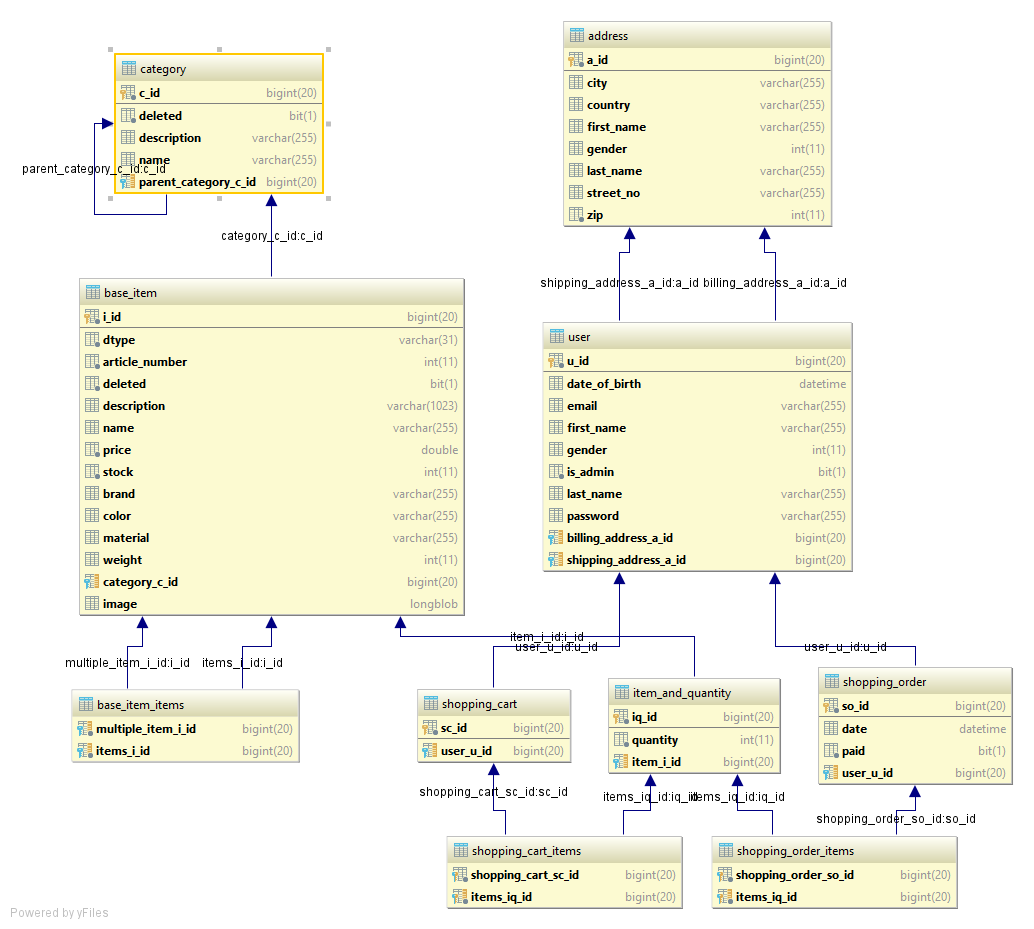
\includegraphics[width=\linewidth]{bilder/kap6/erm_diagram.png}
	\caption{Entity Relationship Modell}
	\label{fig:ERM}
\end{figure}

Die Beziehungen zwischen den Entitäten sind entweder direkt per Fremdschlüssel oder über Beziehungstabellen dargestellt und werden im Folgenden kurz beschrieben.

Ein User hat eine Lieferadresse (Shipping address) und eine Rechnungsadresse (Billing address).
Um die bereits angesprochene Hierarchie von Kategorien abzubilden, können Kategorien eine Eltern-Kategorie haben (Parent category).
Jeder Artikel ist genau einer Kategorie zugeordnet. Für die im Shop so genannten Sets mit mehreren Artikeln, gibt es eine zusätzliche Tabelle, die einem Set mehrere Einzel-Artikel zuordnen kann.
Die Warenkörbe sind immer einem Benutzer zugeordnet. In gleicher Weise sind auch die Bestellungen Benutzer-spezifisch.
Um der Tatsache gerecht zu werden, dass in einem Warenkorb oder in einer Bestellung Artikel mehrmals vorhanden sein können (wenn ein Benutzer von einem Artikel mehrere Exemplare bestellt), wurde eine zusätzliche Entität eingeführt.
Diese \textit{ItemAndQuantity} genannte Entität hält jeweils eine Referenz auf einen Artikel, sowie eine Anzahl für diesen Artikel.
Warenkörbe und Bestellungen enthalten also immer Einträge aus dieser Tabelle.
Auf diese Weise genügt es, für einen Artikel immer nur einen Eintrag zu speichern, auch wenn die bestellte Menge größer ist.
Ohne diese Lösung müsste es für eine Bestellung von beispielsweise dreißig Exemplaren eines Artikels auch dreißig Einträge geben.

\subsection{Design der Weboberfläche}
Vor Beginn der Implementierung wurde ein Konzept für das Design der Weboberfläche erstellt.
Der Fokus lag hierbei eher auf den strukturellen Aspekten der Anwendung, also die Platzierung der unterschiedlichen Elemente auf der Oberfläche, und nicht so sehr auf dem genauen Aussehen dieser Elemente.
Der Grund dafür ist, dass die Struktur einen direkten Einfluss auf die Implementierung der Komponenten hat, während Farben, Schriftarten, Icons usw. auch im Verlauf der Entwicklung ohne einen größeren Umbau verändert werden können.

\cref{fig:mockup_shop} zeigt die grundlegende Struktur der Shop-Oberfläche im Browser.
Wie man sehen kann, ist der Entwurf sehr simpel und intuitiv gehalten. Eine Leiste im Kopfbereich enthält die Links zum Benutzerbereich und zum Warenkorb.
Die größere Menüleiste unter dem Logo erlaubt die Navigation zwischen den Hauptkategorien des Webshops.
Je nachdem in welchem Bereich der Anwendung sich der Benutzer befindet, variiert der Inhalt der Seite.
Prinzipiell soll es fünf unterschiedliche Arten des Inhaltes geben: die Startseite, die Produktlisten zur gewählten Kategorie, die Kontoübersicht, der Warenkorb und die Bestellmaske.
Die Mockups dazu sind im Anhang \ref{appendix:mockups} zu finden.

\begin{figure}[ht!]
	\centering
	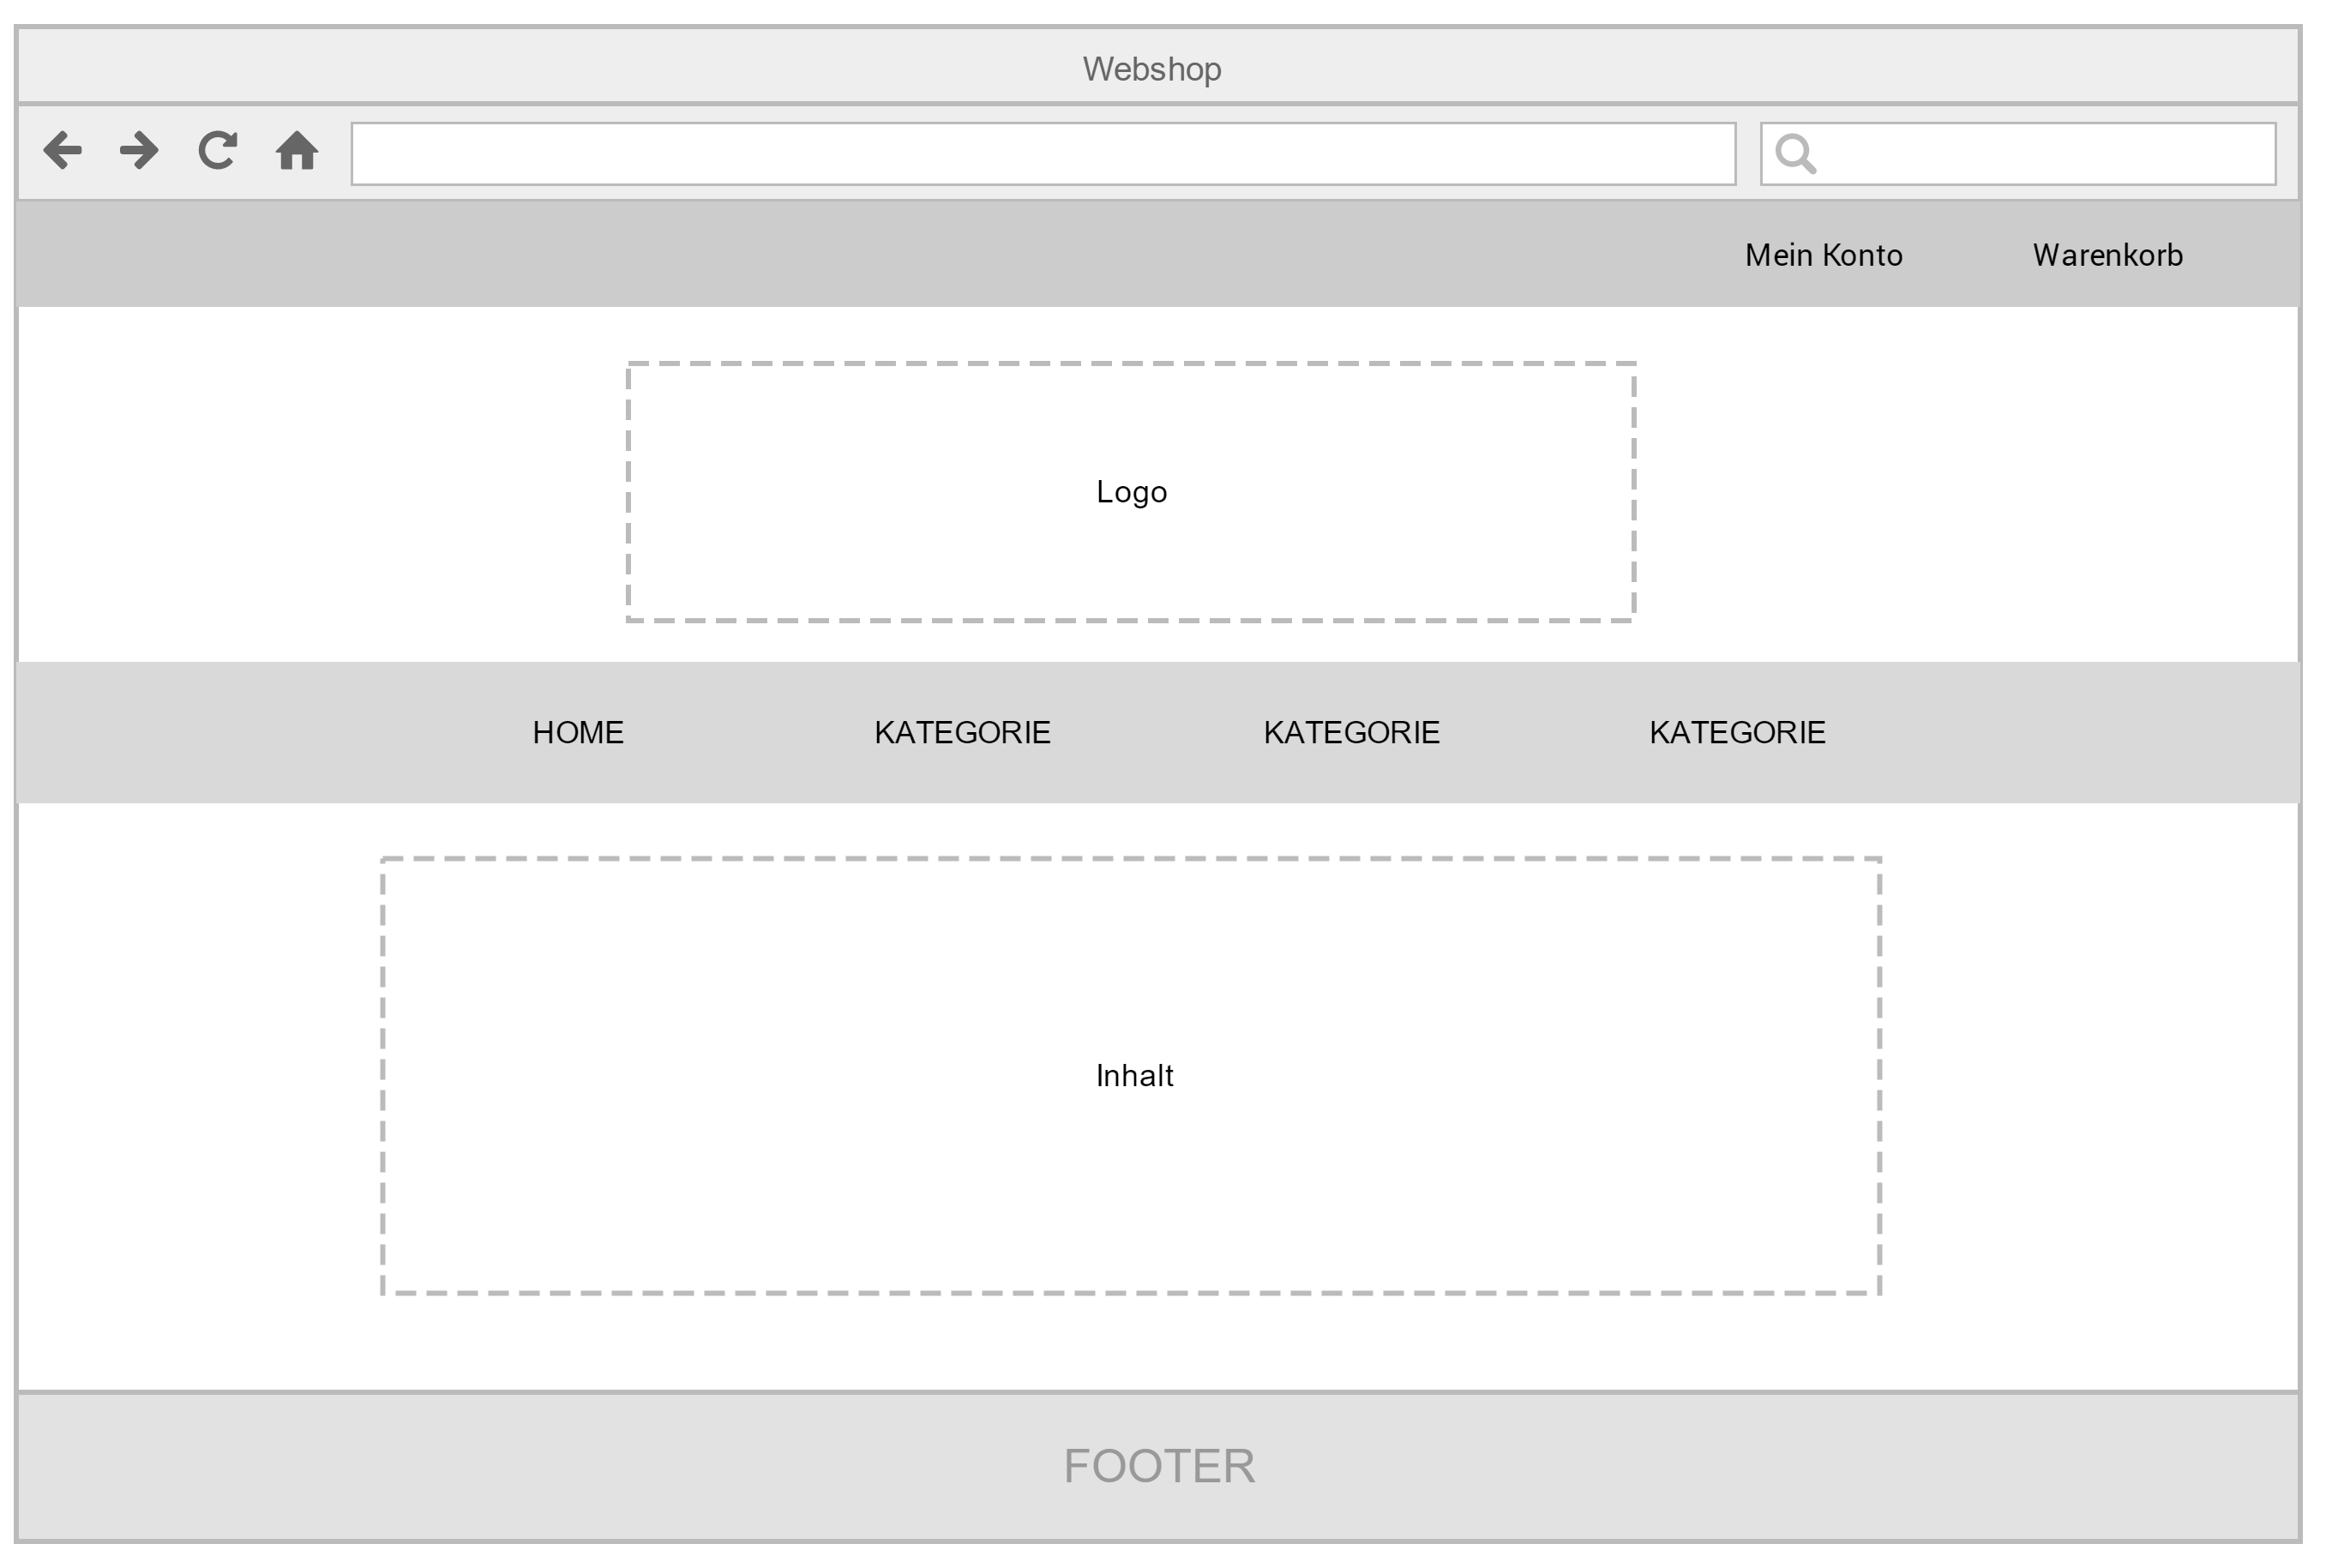
\includegraphics[width=0.8\linewidth]{bilder/kap6/mockup_shop.png}
	\caption{Mockup des Webshops}
	\label{fig:mockup_shop}
\end{figure}

Da eine wachsende Mehrheit der Nutzer mobile Geräte für ihre Internetzugriffe verwendet, ist es sehr wichtig eine Strategie für die Darstellung der Weboberfläche in solchen Geräten zu definieren.
Die in 2016 von der Mediaagentur Zenithmedia veröffentlichte Vorhersage sagte aus, dass in 2017 weltweit 75\% der Internetnutzung über mobile Geräte erfolgen wird, 79\% in 2018 \cite{Zenithmedia2016}.

Es gibt verschiedene Ansätze, um Webseiten für unterschiedliche Displaygrößen zu optimieren.
Eine Möglichkeit wäre es, eine zweite Version der Webseite zu erstellen, welche speziell für die Nutzung auf mobilen Endgeräten angepasst ist.
Eine weitere, modernere Alternative sind Paradigmen wie \textit{Responsive} und \textit{Adaptative} Webdesign.
In beiden Fällen werden sogenannte Breakpoints für die Größe des Displays gesetzt, bei denen die Webseite skaliert und sich an die neue Auflösung anpasst.
Der Unterschied liegt darin, dass beim Adaptative Design eine feste Anzahl an Breakpoints gesetzt wird und es keine Übergänge dazwischen gibt, während beim Responsive Design eine fluide Anpassung auch zwischen den Breakpoints möglich ist.

Der für dieses Projekt gewählte Ansatz ist Responsive Webdesign, da es mithilfe der geplanten Technologien einfach zu realisieren ist.
In \cref{fig:mockup_mobile} ist wieder die Grundstruktur der Webseite zu sehen, jedoch auf die Größe eines Smartphone-Displays skaliert.
Eine wichtige Änderung bei dieser Skalierung betrifft die Menüleiste. Diese sollte nicht länger als Leiste dargestellt werden, sondern als auf- und zuklappbares Dropdown-Menü.
 
\begin{figure}[ht!]
	\centering
	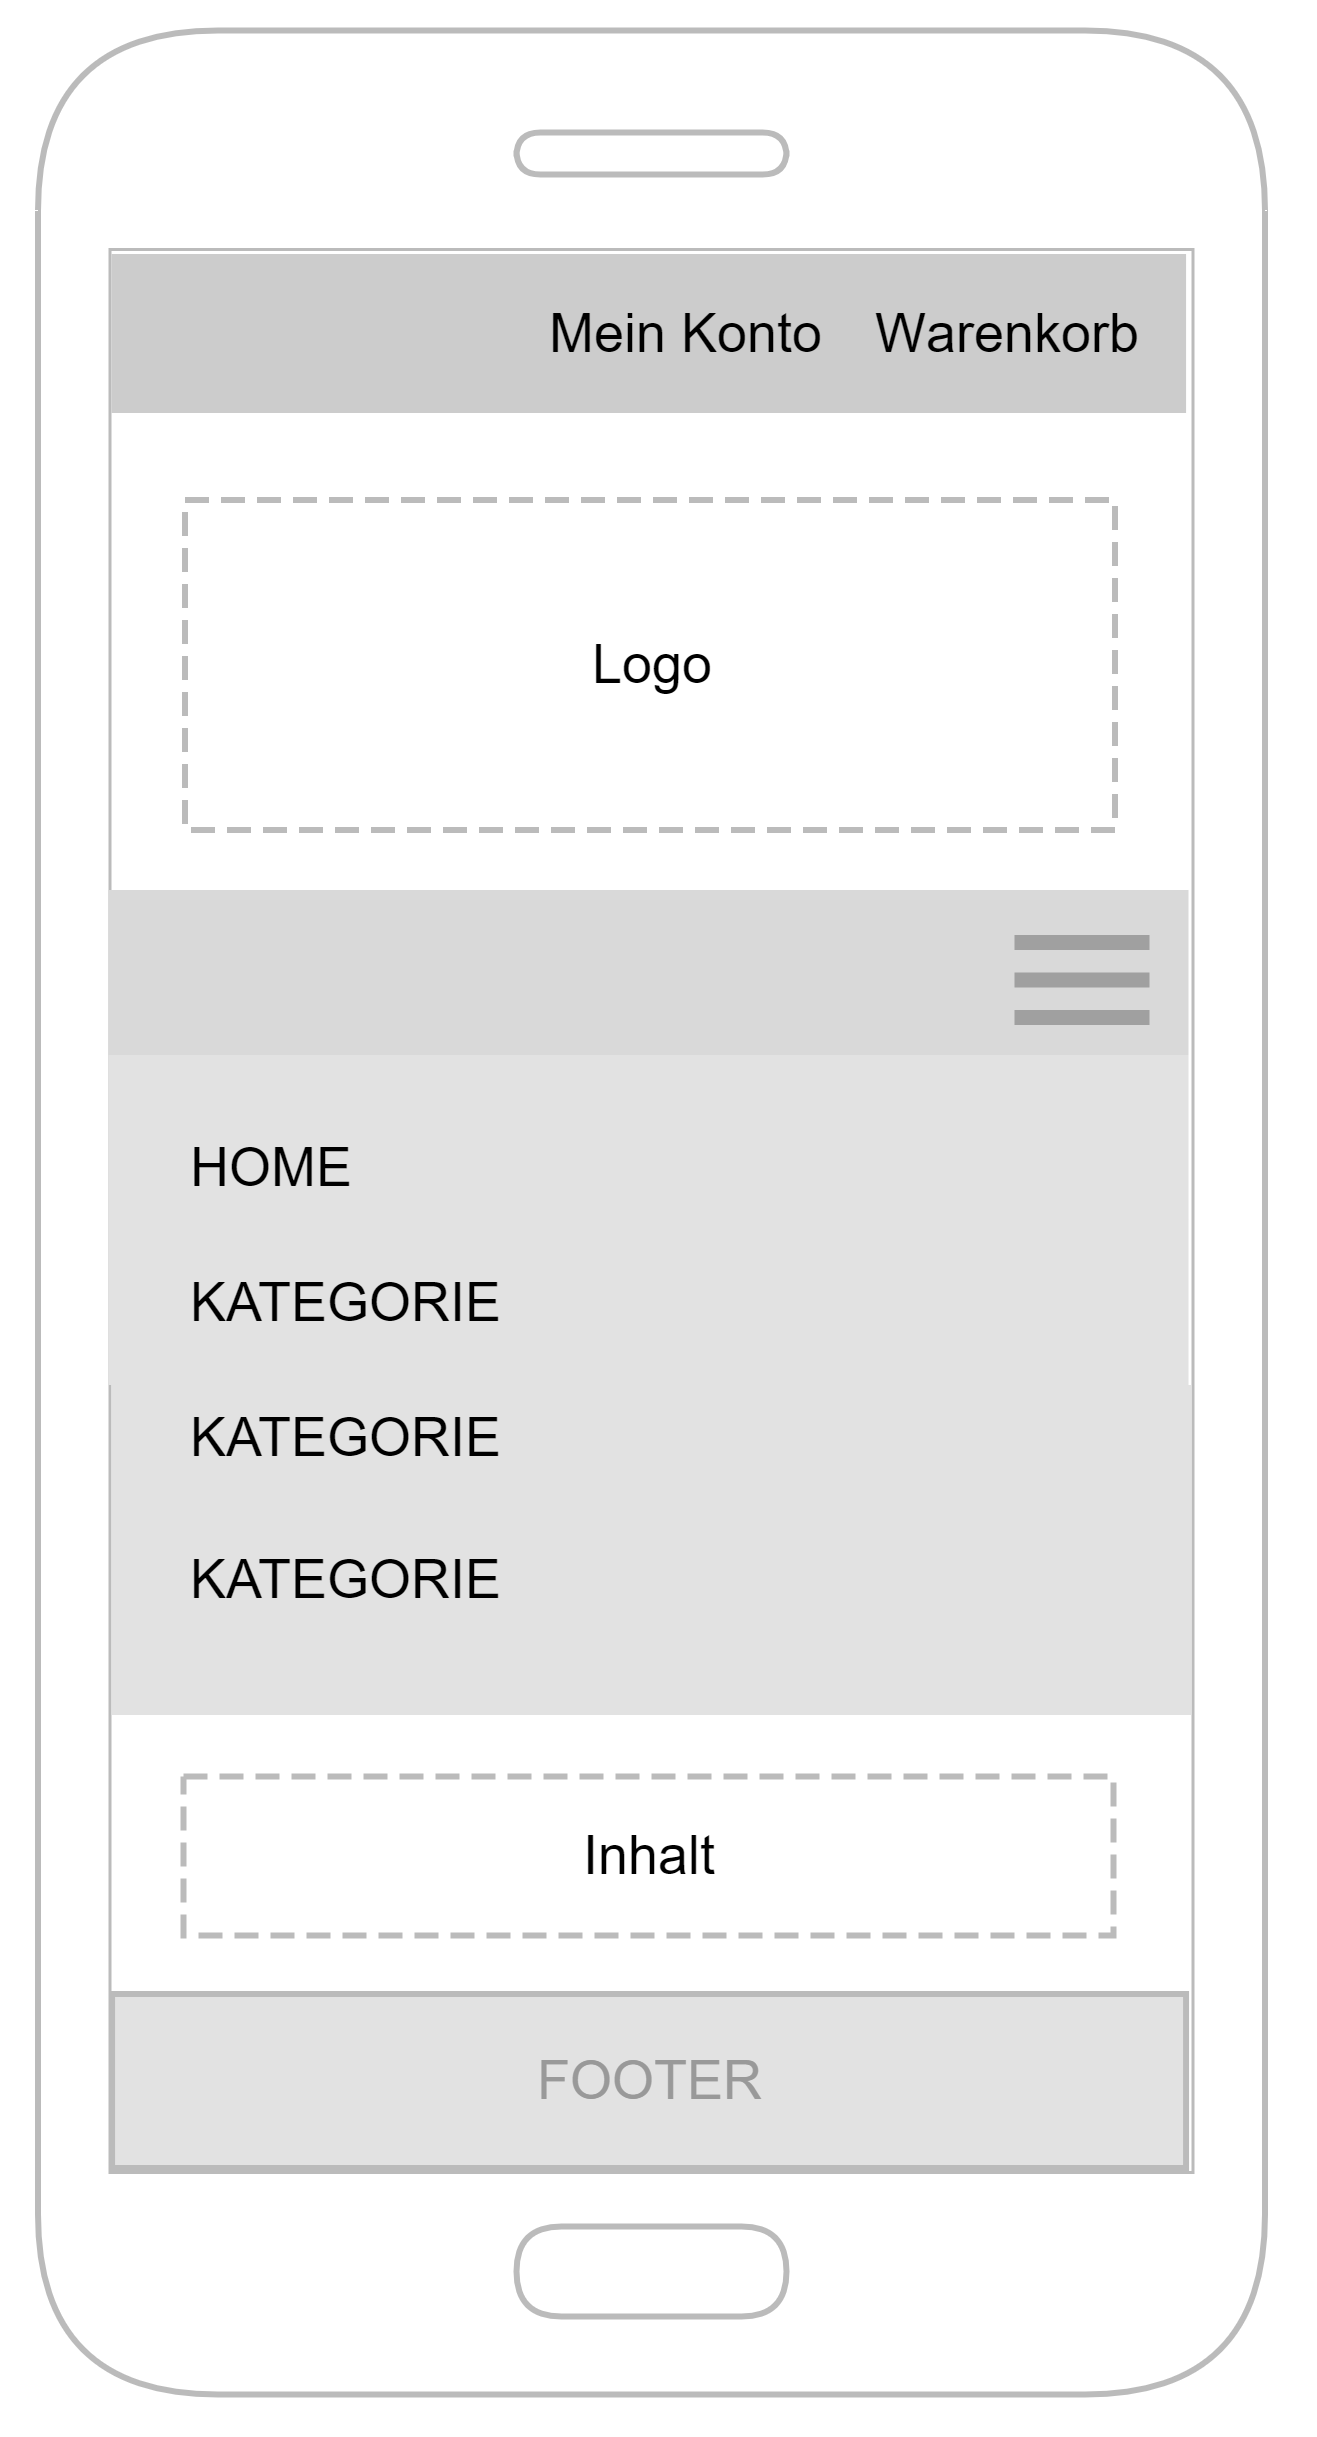
\includegraphics[width=0.25\linewidth]{bilder/kap6/mockup_mobile.png}
	\caption{Mockup des Webshops Handy Version}
	\label{fig:mockup_mobile}
\end{figure}